\documentclass{scrartcl}
\usepackage{mm_ws15}

\newcommand{\permN}{\mathcal{S}_n}
\renewcommand{\mod}{\operatorname{mod}}

% TODO Insert turn-in date
\newcommand{\sheetTitle}{Blatt 1, Abgabe ???}
\newcommand{\uu}{\vec{u}}
\newcommand{\vv}{\vec{v}}
\newcommand{\ww}{\vec{w}}

\begin{document}
\maketitle

\section{Gruppe der Permutationen}
\label{groupperm}
Als Beispiel für eine Gruppe wurde in der Vorlesung die Gruppe der Permutationen von $n$ Elementen $(\permN{}, \ast)$ genannt.
Hierbei ist $\permN$ die Menge aller Anordnungen der Menge $\NN_n = \{1,\ldots,n\}$ (der Menge der natürlichen Zahlen von $1$ bis $n$).
Genauer: $\permN$ ist die Menge der bijektiven (eineindeutigen) Abbildungen von $\NN_n$ auf sich selber.
Die Operation $\ast$ ist definiert durch Hintereinanderausführung der Abbildungen aus $\permN$.
Um die Notation zu vereinfachen werden wir im Weiteren eine Permutation $\sigma \in \permN$ auch als Tupel schreiben $\sigma = (\sigma(1), \sigma(2), \ldots, \sigma(n))$.
Diese Schreibweise spiegelt die äquivalente Charakterisierung von $\permN$ als Menge aller Anordnungen von $n$ Elementen wider.
\begin{subex} 
  \item Für $n=4$ betrachte $\sigma_1 = (2, 4, 1, 3)$, $\sigma_2 = (3, 2, 4 , 1)$ und $\sigma_3 = (2, 1, 3, 2)$.
  Welcher dieser Abbildungen ist keine Permutation?
  Warum?
  Was ist $\sigma_1 \ast \sigma_2$ und $\sigma_2 \ast \sigma_1$?
  Was schlussfolgern Sie daraus für die Gruppe $(\permN,\ast)$?
  \item Beweisen Sie, dass für beliebiges $n \in \NN$, dass $(\permN,\ast)$ eine Gruppe ist.
  \item Beschreiben Sie einen Algorithmus (eine explizite Konstruktionsvorschrift) für $\permN$.
  Mit anderen Worten: gegeben eine Zahl $n$, wie würden Sie alle Elemente aus $\permN$ finden?
  Benutzen Sie \emph{Ihre eigene} Vorschrift um $\mathcal{S}_3$ zu konstruieren!
\end{subex}
\begin{remark}{Hinweis}
  In \ref{groupperm}b) ist die Definition als bijektive Abbildungen von $\NN_n$ nach $\NN_n$ vorteilhaft, für  \ref{groupperm}c) die äquivalente Charakterisierung als Menge aller Anordnungen von $n$ Objekten.
  Beachten Sie für c), dass $\permN$ genau $n! = n \times (n-1) \times \cdots \times 2 \times 1$ Elemente hat.
  Wie kommen die Faktoren zustande?
\end{remark}


\section{Modulare Arithmetik}
Die Menge $\NN_n = \{1,\ldots,n\}$ versehen mit der üblichen Addition $+$ von natürlichen Zahlen bildet keine Gruppe.
Stattdessen definieren die \quotes{Addition modulo $n$} für $a, b \in \NN_n$
\[
a \oplus b = \mod_n(a + b).
\]
\emph{TODO: Erkläre Modulo-Operation, Zeichnung Zahlengerade -> Kreis, Beispiele}
\begin{subex}
  \item Erklären Sie, warum $(\NN_n, +)$ keine Gruppe bildet.
  Ist $(\{0, \ldots, n\},+)$ eine Gruppe?
  \item Sei $n=10$, berechnen Sie $1 \oplus 2$, $3 \oplus 10$ und $4 \oplus 7$.
  \item Beweisen Sie, dass $(\NN_n,\oplus)$ eine Gruppe ist.
  Was ist das neutrale Element?
  Wie lautet das inverse Element für $a\in\NN_n$?
  \item Mit welcher in der Vorlesung bereits behandelten Gruppe können Sie $(\NN_n,\oplus)$ identifizieren?
\end{subex}


\section{Graphische Vektoraddition}
Die in der unten stehenden Abbildung gezeigten Pfeile $\uu, \vv$ und $\ww$ repräsentieren Vektoren, die hier als Verschiebungen in der Ebene zu interpretieren sind.
Skizzieren Sie folgende Linearkombinationen:
\begin{subex}
  \item $\uu + \vv$, $\uu + \ww$, $\uu - \vv$, $\uu - \ww$
  \item $\uu + \vv + \ww -2\ww$, $\frac{1}{2}\uu$, $2\ww + 3(\uu + \vv + \frac{1}{3}\ww)$
\end{subex}
\begin{center}
  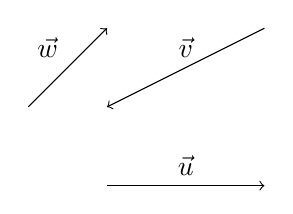
\begin{tikzpicture}[%
    coordline/.style={dotted},
    vector/.style={->}
  ]
      
  \drawgrid{0}{4}{0}{2}
  \draw[vector] (1, 0) -- node[above] {$\uu$} ++ (2,0);
  \draw[vector] (3, 2) -- node[above] {$\vv$} ++ (-2,-1);
  \draw[vector] (0, 1) -- node[above left] {$\ww$} ++ (1,1);

  \end{tikzpicture}
\end{center}

\end{document}